139. \begin{figure}[ht!]
\center{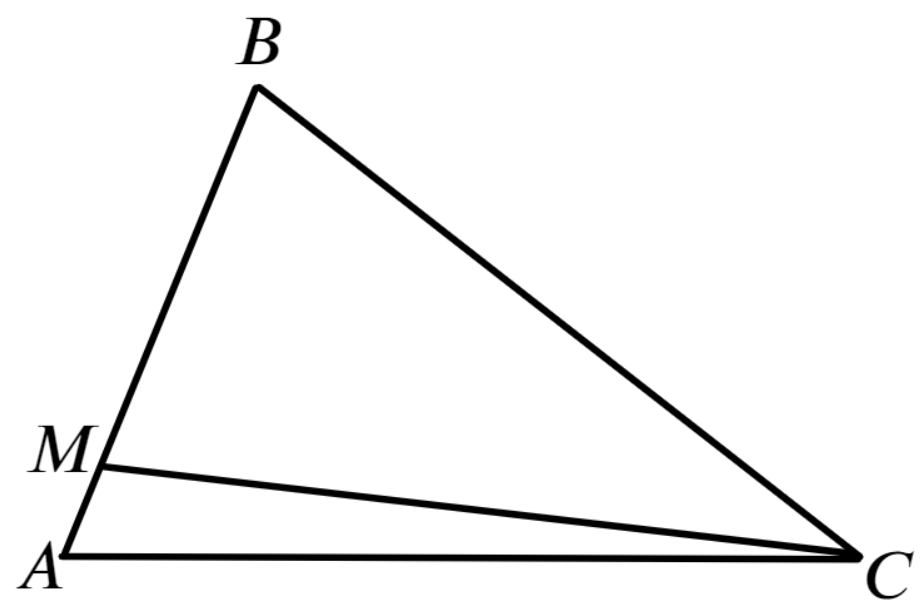
\includegraphics[scale=0.35]{g9-139.png}}
\end{figure}\\
Запишем теорему косинусов для треугольника $ABC:\ 25=36+9-2\cdot6\cdot3\cdot\cos(\angle B),$ откуда $\cos(\angle B)=\cfrac{5}{9}.$ Найдём $BM=\cfrac{5}{6}\cdot6=5$ и запишем теорему косинусов для треугольника $BCM:\ CM^2=9+25-2\cdot3\cdot5\cdot\cfrac{5}{9}=\cfrac{52}{3},$ значит $CM=\cfrac{2\sqrt{39}}{3}.$\\
